\chapter{الكرات النارية، والأطر المرجعية، والمتجهات الرباعية}

نبدأ بسؤال بقي من مناقشة التصادمات عالية الطاقة. فتصادم نواتين ثقيلتين يخلق جسماً يتغير بعنف، لا ثقباً أسود فلكياً هادئاً. فما الذي يمكن أن يعنيه، إذن، وصف هذا التصادم بأفق؟ يقود الجواب عبر صورة خماسية الأبعاد لمادة مقترنة بقوة، ومجموعة من الأسئلة العملية عن المسرّعات، ثم يعود أخيراً إلى هندسة النسبية الخاصة. وبحلول النهاية، تكون السرعة والزخم قد أصبحا متجهين رباعيين، وتكون الطاقة قد أخذت مكانها إلى جانب المركبات الثلاث للزخم.

\section{كرة نارية في بُعد خامس}

\begin{classroomqa}\audiencequestion{الجسم المتولد في التصادم غير مستقر ويتغير شكله. فكيف يمكن تسمية مثل هذا الجسم المعقد ثقباً أسود؟}\lecturerresponse{تخيّل اتجاهاً مكانياً خامساً يمتد بين أرضية وسقف. تجذب الجاذبية في ذلك الاتجاه الاستثارات نحو الأرضية. يودِع التصادم هناك كتلة ساخنة من الطاقة؛ وهذه الكتلة تنتشر ويتغير شكلها، لكنها مع ذلك يمكن أن تمتلك أفقاً ودرجة حرارة وإنتروبيا.}\end{classroomqa}

تخيّل جسيمات، أو على نحو تصويري أكثر أوتاراً صغيرة، تتحرك في هذا العالم الخماسي الأبعاد. فالاستثارات التي تهبط إلى الأرضية تظهر في أربعة أبعاد على هيئة هادرونات: بروتونات ونيوترونات وميزونات وأجسام مركبة ممتدة أخرى. أما الاستثارات المرتبطة بالقرب من السقف فتبدو أكثر أولية. ومن ثم فإن الموضع العمودي طريقة هندسية لترميز المقياس: فالأرضية تمثل النظام الهادروني عند المسافات الطويلة، بينما يمثّل السقف درجات الحرية عند المسافات القصيرة.

عندما يتصادم هادرونان، يصطدم جسمان قرب الأرضية أحدهما بالآخر ويُحدثان تناثراً كبيراً للطاقة. والنتيجة ليست جسماً صلباً. إنها كتلة ساخنة ذات أفق، أشبه ببركة في الحقل الثقالي خماسي الأبعاد. وهي ليست ثقباً أسود فلكياً في الفضاء العادي رباعي الأبعاد، ولا ثقباً أسود على مقياس بلانك ملتصقاً بالسقف. بل هي الوصف الثقالي للكرة النارية شديدة التفاعل قرب الأرضية.

عند الطاقة العالية تنكمش النوى الداخلة انكماش لورنتز إلى أقراص رقيقة. تتصادم، وتودِع طاقتها في منطقة صغيرة، وتنتج مائعاً ينتشر نحو الاتزان. وكانت لزوجته الصغيرة إحدى السمات المفاجئة لبلازما الكوارك--الغلوون. وفي الوصف خماسي الأبعاد يكون التطور نفسه هو استرخاء أفق مشوَّه.

\begin{figure}[H]\centering
\includegraphics[width=0.82\textwidth]{lecture_05_figure_01.png}\caption{تصوّر الأرضية والسقف للبُعد الخامس. تنتشر الكتلة المركزية ذات الأفق على امتداد الأرضية بعد التصادم.}\lectureframe{00:04:22}\end{figure}

لا يبقى الأفق إلى الأبد. فإشعاع هوكينغ يحمل الطاقة بعيداً، وفي الوصف رباعي الأبعاد يكون هذا الإشعاع هو وابل الهادرونات العادية الخارجة من التصادم. وآلاف الآثار في حدث كاشفٍ ما هي، بهذه اللغة، الجسيمات التي تحررت بالغليان من الثقب الأسود النظير.

\subsection{هل البعد الإضافي حقيقي؟}

\begin{classroomqa}\audiencequestion{هل البعد الخامس بُعد مكاني، وهل الخط المرسوم بين الأرضية والسقف يمتد حرفياً في ذلك الاتجاه؟}\lecturerresponse{نعم. إنه من النوع المكاني، والسطح المرسوم في تلك الهندسة الخماسية الأبعاد هو أفق. أمّا ما إذا كان المرء يسمّي الاتجاه الإضافي ``حقيقياً'' أو يعدّه وصفاً رياضياً مكافئاً، فذلك سؤال أعمق.}\end{classroomqa}

والعبارة المفيدة ليست أن الجاذبية تحل محل الديناميكا اللونية الكمومية. بل إن لغتين قد تصفان الفيزياء نفسها. ففي اللغة رباعية الأبعاد توجد كرة نارية ساخنة من الكواركات والغلوونات، من دون حقل ثقالي عادي. وفي اللغة خماسية الأبعاد توجد جاذبية وأفق. وإذا كانت المطابقة صحيحة، فلا بد أن يتفق حساب فعلي في QCD والحساب الثقالي النظير حيثما أمكن إجراء كليهما.

\begin{classroomqa}\audiencequestion{لا توجد في QCD جاذبية ولا آفاق. فهل تضيف صورة الثقب الأسود فيزياء جديدة، أم إنها تعيد فقط وصف الكرة النارية؟}\lecturerresponse{في أربعة أبعاد هي بلازما من الكواركات والغلوونات؛ وفي تمثيلها الخماسي الأبعاد يكون لها وصف ثقالي ذو أفق. والميزة حسابية. فالديناميكا اللونية الكمومية عند الاقتران القوي شديدة الصعوبة، بينما تكون بعض خصائص الأفق---اللزوجة على وجه الخصوص---أسهل حساباً نسبياً.}\end{classroomqa}

لا يلزم حسم التمييز بين ``بُعد حقيقي'' و``تشبيه رياضي'' قبل أن يصبح الوصف مفيداً. وتكتسب بنيةٌ ما تأويلاً فيزيائياً حين تنتظم مع المتغيرات الأخرى في مجموعة أبسط وأكثر تماسكاً من القوانين. ومع ذلك، لا ينبغي المبالغة في الأمر: فتطبيقات ازدواجية العيار/الثقالة على بلازما الكوارك--الغلوون المرصودة هي نماذج لديناميات مقترنة بقوة، لا برهاناً على أن لـ QCD في العالم الواقعي نظيراً ثقالياً دقيقاً معروفاً.\editorialnote{يجعل هذا التقييد الوضع الحديث لتطبيق QCD صريحاً؛ وهو لا يغيّر الآلية الخماسية الأبعاد المطوَّرة هنا.}

\section{لماذا تستخدم المصادمات حُزَماً متصادمة}

تصبح الأسئلة الآن عملية. لماذا نستخدم حزمتين متحركتين بدلاً من حزمة واحدة وهدف ساكن؟ ولماذا تكون المسرّعات الدائرية كبيرة إلى هذا الحد؟ ولماذا يُتعامل مع الإلكترونات والبروتونات على نحو مختلف؟ كل هذه الأسئلة هي أسئلة عن الطاقة النسبية.

\begin{classroomqa}\audiencequestion{لماذا نُصادِم حزمتين بدلاً من إطلاق حزمة عالية الطاقة واحدة على هدف ساكن؟}\lecturerresponse{الذي يخلق جسيمات جديدة هو الطاقة المتاحة في إطار مركز الكتلة. فحزمتان نسبيتان متساويتان ومتعاكستان لا تملكان زخماً صافياً، لذا تكون كل طاقتهما تقريباً متاحة للتصادم. أما الهدف الثابت فيجبر كثيراً من الطاقة الساقطة على أن تبقى على هيئة حركة لمركز الكتلة.}\end{classroomqa}

بالنسبة إلى جسيمين فائقَي النسبية لهما زخمان متعاكسان مقدار كل منهما \(p\)، فإن التقدير على مستوى المحاضرة في وحدات \(c=1\) هو \begin{equation}
E_{\mathrm{cm}}^{\mathrm{collider}}\simeq 2p.
\end{equation} أما التقدير المناظر لحالة الهدف الثابت فلا ينمو إلا مثل الجذر التربيعي لزخم الحزمة، \begin{equation}
E_{\mathrm{cm}}^{\mathrm{fixed}}\sim \sqrt{mp}.
\end{equation} والمغزى هو كيفية التدرج، لا العامل العددي المُهمَل: فمضاعفة طاقة الحزمة تضاعف طاقة المصادم، لكنها لا تزيد طاقة مركز الكتلة في حالة الهدف الثابت إلا وفق جذر تربيعي.

يجعل الحساب اللابدي المقارنة دقيقة. فإذا كان \(P_1\) و\(P_2\) هما رباعيي الزخم الداخلين، فإن \begin{equation}
s=(P_1+P_2)^2,
\qquad E_{\mathrm{cm}}=\sqrt{s}.
\end{equation} وبالنسبة إلى حزمتين متساويتين متعاكستي الاتجاه طاقة كل منهما \(E\)، فإن مركبات الزخم المكانية تتلاشى ويكون \(\sqrt{s}=2E\). أمّا لمقذوف طاقته \(E\gg m\) يصطدم بهدف ساكن مساوي له في الكتلة، فإن \begin{equation}
s=2m^2+2mE,
\qquad
\sqrt{s}\simeq \sqrt{2mE}
\qquad (c=1).
\end{equation} وهذا الاشتقاق اللابدي القصير يزوّدنا بالعامل الذي حُذف في التقدير الشفهي.\editorialnote{أُدرج هذا الاشتقاق لكي يمكن إعادة إنتاج حجة التدرج الواردة في المحاضرة.}

\begin{classroomqa}\audiencequestion{هل هناك سبب أساسي يجعل المسرّع الدائري لا بد أن يكون كبيراً إلى هذا الحد؟ أما كان يمكن للحزمة نفسها أن تدور ببساطة في آلة أصغر عدداً أكبر من المرات؟}\lecturerresponse{تفرض الحقول والمواد حدوداً. فالجسيم يتلقى زيادة محدودة في الطاقة لكل متر، لذا تحتاج الآلة الأعلى طاقة إلى طول تسريع فعّال أكبر. كما أن الدائرة الضيقة تتطلب تسارعاً مستعرضاً أكبر، والشحنة المتسارعة تشع. وإذا كانت الحلقة صغيرة أكثر مما ينبغي، تشع الحزمة طاقة بالسرعة نفسها التي تمدها بها الآلة.}\end{classroomqa}

وعلاقة الانحناء تقريباً هي \begin{equation}
p=qBR,
\end{equation} لذا، عند تثبيت المجال المغناطيسي \(B\)، يتطلب زخم أكبر \(p\) نصف قطر أكبر \(R\). وتؤدي تجاويف الترددات الراديوية الشغل الذي يرفع طاقة الحزمة؛ والمغناطيسات تثني الحزمة وتُركّزها. وتبقى الخلاصة العامة هي نفسها التي عُرضت على اللوح: فقوة الحقل وفواقد الإشعاع تمنعاننا من ضغط مسرّع ذي طاقة مهما ارتفعت في حلقة صغيرة.

تنطوي الحركة الدائرية على تسارع حتى عند ثبات السرعة، لأن متجه السرعة يغيّر اتجاهه. والشحنة المتسارعة تبعث إشعاعاً سنكروترونياً. ويتجنب المسرّع الخطي فاقد الانحناء المستمر، مع أن دفعات التسريع القصيرة نفسها ليست، حرفياً، خاليةً من الإشعاع. وتقبل الآلات الدائرية كلفة الانحناء مقابل إعادة استخدام الجهاز نفسه في كل دورة.

\begin{classroomqa}\audiencequestion{لماذا ارتبطت الإلكترونات بالآلة المستقيمة في SLAC بينما تستخدم المصادمات الدائرية عالية الطاقة بروتونات أو هادرونات أخرى؟}\lecturerresponse{الإلكترونات أخف بكثير. فعند طاقة عالية معطاة يكون عامل لورنتز لديها أكبر بكثير، ويجعلها التسارع الدائري تشع على نحو أشد كثيراً. أمّا البروتونات الأثقل فتستطيع أن تدور مراراً، مكتسبة طاقة في كل مرور، قبل أن تصبح فواقد الإشعاع السنكروتروني باهظةً بحيث تمنع ذلك.}\end{classroomqa}

عند ثبات الطاقة ونصف قطر الحلقة، تعتمد القدرة المشعّة اعتمادًا حادًا جدًا على كتلة الجسيم،
\begin{equation}
P_{\mathrm{sync}}\propto \frac{E^4}{m^4R^2}.
\end{equation}
ولهذا فإن الفارق بين الإلكترون--البروتون أشد بكثير مما قد توحي به العبارة ``الجسيم الأخف يتحرك أسرع'': فقد تكون كلتا الحزمتين قريبتين للغاية بالفعل من \(c\)، لكن معاملي لورنتز وخسائر الإشعاع فيهما مختلفان جدًا.\editorialnote{إن علاقة الانحناء وتحجيم الإشعاع السنكروتروني يجعلان الحجة النوعية الخاصة بالمسرِّعات في المحاضرة دقيقة؛ ولم يُجرِ تفصيلهما على اللوح.}

\begin{classroomqa}
\audiencequestion{لماذا لا نُسرِّع الهادرونات في خط مستقيم أيضًا؟}
\lecturerresponse{يمكن ذلك. الصعوبة هي الطول. ففي الحلقة يمر الجسيم نفسه عبر بُنى التسريع مرات كثيرة؛ أما آلة هادرونات خطية مكافئة فستحتاج إلى أن تكون طويلة على نحو هائل. والحل الوسط العملي هو حلقة كبيرة، كبيرة بما يكفي لكي يبقى إشعاع البروتون مقبولًا.}
\end{classroomqa}

تكشف هذه الأسئلة المتعلقة بالمسرِّعات على وجه الدقة لماذا لا تكفي القواعد النيوتنية. ونعود الآن إلى النسبية الخاصة ونبني اللغة التي تجعل مثل هذه المقارنات ممنهجة.

\section{المرأب والليموزين}

تأمل مرأبًا طوله نحو اثني عشر قدمًا وسيارة ليموزين طويلة طولها نحو عشرين قدمًا. يزيد السائق السرعة حتى تصبح الليموزين منكمشة انكماش لورنتز، آملًا أن تتسع لها. في إطار المرأب تكون الليموزين المتحركة أقصر، لذا يبدو ذلك ممكنًا. لكن في إطار الليموزين يكون المرأب المتحرك أقصر، لذا يبدو ذلك مستحيلًا. هل يمكن أن تكون الليموزين كلها داخل المرأب؟

افتح البابين كليهما حتى لا يشتتنا أي اصطدام بجدار. والقول إن الليموزين في الداخل يعني أن مقدمتها ومؤخرتها في الداخل \emph{في آن واحد}. وهذه الكلمة الأخيرة تتضمن اللغز كله.

ارسم مخططًا للزمكان يكون فيه \(t\) عموديًا و\(x\) أفقيًا. وتشكل أشعة الضوء مخروط الضوء ذي زاوية \(45^\circ\) في وحدات \(c=1\). المرأب ساكن، لذا فإن خطي العالم لبابيه عموديان. وترسم مقدمة الليموزين ومؤخرتها خطي عالم مائلين متوازيين. ويميل محور \(t'\) للإطار المتحرك نحو مخروط الضوء، وخطوط التزامن فيه موازية لمحور \(x'\) المائل.

\begin{figure}[H]
\centering
\includegraphics[width=0.82\textwidth]{lecture_05_figure_02.png}
\caption{مخطط الزمكان المكتمل للمرأب--الليموزين. تحد الخطوط العمودية المرأب؛ وتتبع الخطوط المائلة طرفي الليموزين. وتمثل المقاطع الأفقية والمائلة شرائح التزامن المختلفة في الإطارين.}
\lectureframe{00:31:05}
\end{figure}

في إطار المرأب، يمكن لخط أفقي أن يقطع خطي عالم الليموزين كليهما بين خطي عالم المرأب. وعند تلك اللحظة في المرأب تكون المؤخرة قد دخلت ولم تكن المقدمة قد خرجت بعد. وتكون الليموزين المنكمشة كلها في الداخل.

في إطار الليموزين، تقع الأحداث المتزامنة المعنية على خط مائل. ارسم خطًا من هذا النوع يمر بالحدث الذي تدخل عنده المؤخرة. وهو يلتقي بخط عالم المقدمة بعد أن تكون المقدمة قد تجاوزت الباب البعيد بالفعل. ووفقًا لتزامنها الخاص، لا تكون الليموزين بكاملها في الداخل أبدًا. وكلتا العبارتين صحيحتان لأنهما تقارنان بين زوجين مختلفين من الأحداث.

\begin{classroomqa}
\audiencequestion{هل يشكّل خطا العالم الأخضران والمقطع الأفقي بينهما متوازي أضلاع؟ وهل ذلك المقطع الأسود هو طول المركبة؟}
\lecturerresponse{المقطع الأفقي هو الطول المنكمش بلورنتز، لأن طرفيه متزامنان في إطار المرأب. ويُستحصل على الطول الذاتي من طرفين متزامنين في إطار الليموزين، على خط موازٍ لـ \(x'\). ويستخدم القياسان قطعين مختلفين عبر الزوج نفسه من خطّي العالم.}
\end{classroomqa}

إذا كان \(L_0\) هو الطول الذاتي، فإن طول القطع الأفقي في إطار المرأب هو
\begin{equation}
L=\frac{L_0}{\gamma},
\qquad
\gamma=\frac{1}{\sqrt{1-v^2/c^2}}.
\end{equation}
المعادلة وحدها لا تحل المفارقة. بل يفعل ذلك الرسم، لأنه يبين أيَّ الأحداث قد قورنت. وكلما بدت مسألة في النسبية وكأنها تُنتج جوابين غير متوافقين، فابحث عن استعمال غير مصرَّح به للتعبير ``في الوقت نفسه''.

\section{أربعة إحداثيات وموضعان للمؤشر}

للانتقال من المفارقات إلى قوانين الحركة، نحتاج إلى ترميز يحفظ البنية الهندسية. نجمع الإحداثيات في الصورة
\begin{equation}
(X^1,X^2,X^3,X^0)=(x,y,z,t),
\qquad X^\mu=(x,y,z,t),
\end{equation}
حيث يأخذ \(\mu\) القيم \(1,2,3,0\). ويضع هذا الترتيب الزمن أخيرًا على الصفحة، مع أن مؤشِّره هو \(0\)، موافقًا للاصطلاح المستخدم على السبورة.

\begin{classroomqa}
\audiencequestion{هل نأخذ \(c=1\)؟ وإذا أُعيدت الوحدات العادية، فهل ينبغي أن يكون إحداثي الزمن هو \(ct\)؟}
\lecturerresponse{نعم. نأخذ \(c=1\) أثناء تطوير الهندسة، ونعيد عوامل \(c\) عندما تكون الأبعاد أو الحد غير النسبي مهمَّين. ومع وحدات الطول المألوفة، يكون إحداثي الزمن هو \(ct\).}
\end{classroomqa}

يمكن كتابة المتجه نفسه بمؤشر سفلي. ووفق اصطلاح الإشارة المستخدم هنا،
\begin{equation}
X_\mu=(-x,-y,-z,t).
\end{equation}
ومن ثم فإن إنزال المؤشر يعكس إشارات المركبات المكانية الثلاث ويترك مركبة الزمن من دون تغيير. على سبيل المثال،
\begin{equation}
X^\mu=(3,2,4,10)
\quad\Longrightarrow\quad
X_\mu=(-3,-2,-4,10).
\end{equation}
وهذان ليسا نقطتين في الزمكان؛ بل صورتان بالمركبات لكائن هندسي واحد.

\begin{classroomqa}
\audiencequestion{أيُّ المركبات موافقة التباين وأيُّها مخالفة التباين، وهل يُراد بالعلامات أن تكون مؤشرات علوية أم سفلية؟}
\lecturerresponse{المركبات ذات المؤشر العلوي مخالفة التباين؛ وذات المؤشر السفلي موافقة التباين. ومن وسائل التذكّر المفيدة في القاعة أن ``co منخفض، contra مرتفع''. وكثيرًا ما يقول الفيزيائيون ببساطة: في الأعلى وفي الأسفل.}
\end{classroomqa}

تبرز جدوى هذا الترميز في الانكماش الثابت
\begin{equation}
X_\mu X^\mu=t^2-x^2-y^2-z^2.
\label{eq:l5-interval}
\end{equation}
وفي الصيغة التفاضلية يصبح هذا
\begin{equation}
d\tau^2=dt^2-dx^2-dy^2-dz^2
\qquad (c=1).
\label{eq:l5-proper-time}
\end{equation}
وبالنسبة إلى حركة زمنية، فإن \(d\tau\) هو الزمن الذي تسجله ساعة تتحرك على طول خط العالم.

كلما ظهر المؤشر نفسه مرةً علويًا ومرةً سفليًا، فالمفهوم أنه يُجمع عليه. ويحوِّل اصطلاح آينشتاين
\begin{equation}
\sum_{\mu}X_\mu X^\mu
\end{equation}
إلى التعبير الأقصر في المعادلة ~\eqref{eq:l5-interval}. وليس هذا مجرد اختصار طباعي، بل إنه يحول دون إعادة كتابة الإشارات المتناوبة في هندسة مينكوفسكي يدويًا في كل معادلة.

\begin{classroomqa}
\audiencequestion{هل \(\tau\) هو الرمز القياسي للزمن الذاتي؟}
\lecturerresponse{نعم. ويُستخدم الرمز \(s\) أيضًا أحيانًا، لكن \(\tau\) اختيار قياسي للزمن الذاتي.}
\end{classroomqa}

\section{الدورانات بوصفها التناظر الأسهل}

يخلط التحويل الدفعي اللورنتزي بين المكان والزمان. قبل أن ندرس تلك المصفوفة، فلننظر إلى العملية الأكثر ألفة، وهي تدوير المحاور المكانية. إذا كان اتجاه الحركة النسبية اعتباطيًا، أمكننا تدوير المحاور حتى يغدو ذلك الاتجاه هو المحور \(x\) الجديد، ثم نطبق التحويل الدفعي المعروف. ولذلك فالدورانات جزء من البناء، وليست مجرد استطراد للزينة.

لدوران بزاوية \(\theta\) حول المحور \(z\)،
\begin{align}
x'&=x\cos\theta+y\sin\theta,\nonumber\\
y'&=-x\sin\theta+y\cos\theta,\label{eq:l5-rotation}\\
z'&=z.\nonumber
\end{align}
عند \(\theta=0\) تعطي هذه المعادلات \(x'=x\) و\(y'=y\)؛ وعند \(\theta=\pi/2\) تعطي تبادلًا بين الإحداثيات مع الإشارات المتوقعة.

يحفظ هذا التحويل المسافة الإقليدية. وإذا كتبنا \(c_\theta=\cos\theta\) و\(s_\theta=\sin\theta\)،
\begin{align}
x'^2+y'^2
&=(xc_\theta+ys_\theta)^2+(-xs_\theta+yc_\theta)^2\nonumber\\
&=x^2(c_\theta^2+s_\theta^2)
  +y^2(s_\theta^2+c_\theta^2)\nonumber\\
&\quad+2xyc_\theta s_\theta-2xyc_\theta s_\theta\nonumber\\
&=x^2+y^2.
\end{align}
فإن الحدود المختلطة تتلاشى، و\(c_\theta^2+s_\theta^2=1\). وبما أن \(z'=z\)، فإن الطول الكلي \(x^2+y^2+z^2\) ثابت.

يمكن كتابة هذه المعادلات في صورة معادلة مصفوفية واحدة:
\begin{equation}
\begin{pmatrix}x'\\y'\\z'\end{pmatrix}
=
\underbrace{\begin{pmatrix}
\cos\theta&\sin\theta&0\\
-\sin\theta&\cos\theta&0\\
0&0&1
\end{pmatrix}}_{M}
\begin{pmatrix}x\\y\\z\end{pmatrix}.
\label{eq:l5-rotation-matrix}
\end{equation}
وبترميز المؤشرات،
\begin{equation}
x'^i=M^i{}_{j}x^j,
\qquad i,j=1,2,3.
\end{equation}

\begin{figure}[H]
\centering
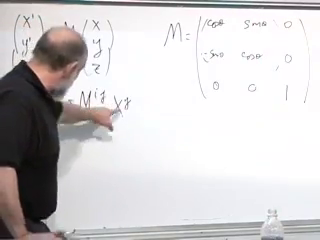
\includegraphics[width=0.82\textwidth]{lecture_05_figure_03.png}
\caption{الدوران المكاني مكتوبًا على هيئة معادلة مصفوفية وبترميز المؤشرات معًا.}
\lectureframe{01:00:40}
\end{figure}

\section{مصفوفات لورنتز وتركيب السرعات}

لحركة على طول \(x\)، يكون تحويل لورنتز في وحدات \(c=1\) هو
\begin{align}
x'&=\gamma_v(x-vt), & y'&=y,\nonumber\\
z'&=z, & t'&=\gamma_v(t-vx),
\end{align}
حيث
\begin{equation}
\gamma_v=\frac{1}{\sqrt{1-v^2}}.
\end{equation}
ومع ترتيب المركبات \((x,y,z,t)\)، يصبح ذلك
\begin{equation}
\begin{pmatrix}x'\\y'\\z'\\t'\end{pmatrix}
=
\begin{pmatrix}
\gamma_v&0&0&-\gamma_vv\\
0&1&0&0\\
0&0&1&0\\
-\gamma_vv&0&0&\gamma_v
\end{pmatrix}
\begin{pmatrix}x\\y\\z\\t\end{pmatrix}.
\label{eq:l5-lorentz-matrix}
\end{equation}

\begin{figure}[H]
\centering
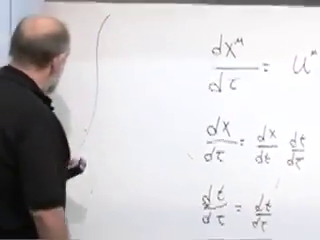
\includegraphics[width=0.82\textwidth]{lecture_05_figure_04.png}
\caption{مصفوفة لورنتز \(4\times4\). تختلط فقط المركبتان \(x\) و\(t\)؛ أما \(y\) و\(z\) فتبقيان دون تغير.}
\lectureframe{01:04:40}
\end{figure}

تجيب عملية ضرب المصفوفات الآن عن سؤال فيزيائي. افترض أن راصدًا يتحرك بسرعة \(v\) بالنسبة إلينا، وأن راصدًا ثالثًا يتحرك بسرعة \(u\) بالنسبة إلى ذلك الراصد، وجميع هذه الحركات على المحور نفسه. أما الحركيات النيوتونية فكانت ستعطي \(w=u+v\)، مما كان سيسمح بأن تتركب سرعتان كل منهما \(3c/4\) إلى \(3c/2\). لا بد أن تعطي النسبية قاعدة مختلفة.

الجزء الفعّال من تحويلة الدفع هو المصفوفة \(2\times2\)
\begin{equation}
B(v)=\gamma_v
\begin{pmatrix}1&-v\\-v&1\end{pmatrix}.
\end{equation}
ويعطي تركيب تحويلتي الدفع
\begin{align}
B(u)B(v)
&=\gamma_u\gamma_v
\begin{pmatrix}1&-u\\-u&1\end{pmatrix}
\begin{pmatrix}1&-v\\-v&1\end{pmatrix}\nonumber\\
&=\gamma_u\gamma_v
\begin{pmatrix}
1+uv&-(u+v)\\
-(u+v)&1+uv
\end{pmatrix}.
\label{eq:l5-composed-boost}
\end{align}
وتحدِّد نسبةُ مدخلٍ غير قطري إلى مدخلٍ قطري سرعةَ تحويلة الدفع الناتجة:
\begin{equation}
w=\frac{u+v}{1+uv}
\qquad(c=1).
\end{equation}
وبإعادة الأبعاد،
\begin{equation}
w=\frac{u+v}{1+uv/c^2}.
\label{eq:l5-velocity-addition}
\end{equation}

\begin{figure}[H]
\centering
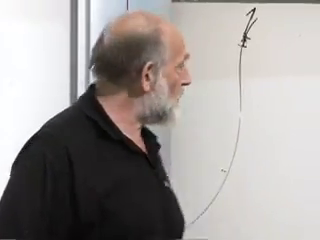
\includegraphics[width=0.82\textwidth]{lecture_05_figure_05.png}
\caption{مصفوفة تحويلة الدفع المركبة والسرعة
\(w=(u+v)/(1+uv)\) في الوحدات الطبيعية.}
\lectureframe{01:15:35}
\end{figure}

إذا كان كلٌّ من \(u\) و\(v\) قريبًا من \(c\)، فإن البسط يقترب من \(2c\)
بينما يقترب المقام من \(2\)، لذا تقترب \(w\) من \(c\)، لا من
\(2c\). وعلى نحو أعم، فإن المعادلة ~\eqref{eq:l5-velocity-addition} تحوِّل المدخلات دون الضوئية
إلى نتيجة دون ضوئية. وقد ضمَّنت عملية ضرب المصفوفات حدَّ السرعة
تلقائيًا.

\section{المتجهات الرباعية وفشل السرعة العادية}

المتجه الرباعي هو أي كائن تتحول مركباته الأربع تحت الدورانات
والدفعات اللورنتزية بالطريقة نفسها التي تتحول بها إحداثيات الزمكان. إذا كان \(V^\mu\)
متجهًا رباعيًا، فعند اعتماد اصطلاح الإشارة لدينا
\begin{equation}
V_\mu=(-V^1,-V^2,-V^3,V^0),
\end{equation}
ويكون معياره الثابت
\begin{equation}
V_\mu V^\mu=(V^0)^2-(V^1)^2-(V^2)^2-(V^3)^2.
\end{equation}
وبالنسبة إلى المتجهين الرباعيين \(V^\mu\) و\(W^\mu\)، فإن الانكماش
\begin{equation}
W_\mu V^\mu
=W^0V^0-W^1V^1-W^2V^2-W^3V^3
\end{equation}
هو أيضًا ثابت. تتغير المركبات من إطار مرجعي إلى آخر؛ أما الانكماش فلا يتغير.

للسرعة العادية ثلاث مركبات فقط،
\begin{equation}
\mathbf v=\left(\frac{dx}{dt},\frac{dy}{dt},\frac{dz}{dt}\right).
\end{equation}
وإلحاق \(dt/dt=1\) بها لا يجعلها متجهًا رباعيًا مفيدًا. فالمركبة الرابعة
ستكون تافهة، ولن يتحول الكائن الناتج خطيًا تحت
تحويلات لورنتز. يتغير الزمن الإحداثي \(t\) من إطار مرجعي إلى
آخر، لذلك فإن الاشتقاق بالنسبة إلى \(t\) يفسد قانون التحول المطلوب.

يوفّر الزمن الخاص الحل. على طول خط عالم نعرّف
\begin{equation}
u^\mu=\frac{dX^\mu}{d\tau}.
\label{eq:l5-four-velocity}
\end{equation}
التفاضل \(dX^\mu\) متجه رباعي و\(d\tau\) مقدار ثابت، لذا فإن
نسبتهما متجه رباعي. وتشير الصفة ``الخاص'' إلى الساعة الواردة في
المقام.

تربط قاعدة السلسلة هذا المقدار بالسرعة العادية:
\begin{equation}
\frac{dx}{d\tau}=\frac{dx}{dt}\frac{dt}{d\tau},
\end{equation}
وبالمثل بالنسبة إلى \(y\) و\(z\). من
المعادلة ~\eqref{eq:l5-proper-time}،
\begin{align}
\left(\frac{d\tau}{dt}\right)^2
&=1-\left(\frac{dx}{dt}\right)^2
    -\left(\frac{dy}{dt}\right)^2
    -\left(\frac{dz}{dt}\right)^2\nonumber\\
&=1-v^2
\qquad(c=1),
\end{align}
ومن ثم
\begin{equation}
\frac{dt}{d\tau}=\gamma_v=\frac{1}{\sqrt{1-v^2}}.
\end{equation}
والمركبات الأربع هي
\begin{equation}
u^i=\gamma_v v^i,
\qquad
u^0=\gamma_v
\qquad(c=1).
\label{eq:l5-four-velocity-components}
\end{equation}
عند السرعة الصغيرة، يكون \(u^i\simeq v^i\) و\(u^0\simeq1\). وأما قرب سرعة الضوء،
فإن \(\gamma_v\) يزداد بلا حد وتختلف السرعة الخاصة اختلافًا حادًا عن
السرعة العادية.

\begin{figure}[H]
\centering
\includegraphics[width=0.82\textwidth]{lecture_05_figure_06.png}
\caption{المركبات الأربع للسرعة الخاصة معبَّرًا عنها بدلالة السرعة العادية وعامل لورنتز.}
\lectureframe{01:34:40}
\end{figure}

بإرجاع الوحدات التقليدية واستخدام \(X^0=ct\) نحصل على الصورة القياسية
\begin{equation}
U^\mu=(\gamma_v\mathbf v,\gamma_v c)
\end{equation}
في الترتيب المستخدم هنا الذي تُقدَّم فيه المركبات المكانية أولًا. ومعياره الثابت هو
\begin{equation}
U_\mu U^\mu=c^2.
\end{equation}
وعليه، فلكل جسيم ذي كتلة سرعة رباعية لها المقدار الثابت نفسه، مع أن
سرعته المكانية تعتمد على الإطار المرجعي.

\section{المماس لخط العالم}

يوجد نظير إقليدي مألوف للمعادلة ~\eqref{eq:l5-four-velocity}.
فعلى طول منحنى في الفضاء الثلاثي الأبعاد العادي،
\begin{equation}
ds^2=dx^2+dy^2+dz^2.
\end{equation}
تشير الإزاحة التفاضلية \((dx,dy,dz)\) على امتداد المنحنى لكنها
ليست متجه وحدة. وبالقسمة على طول القوس نحصل على
\begin{equation}
\mathbf T=
\left(\frac{dx}{ds},\frac{dy}{ds},\frac{dz}{ds}\right),
\qquad
\mathbf T\cdot\mathbf T=1.
\end{equation}
والبناء النسبي هو الفكرة نفسها مع الزمن الخاص بدلًا من طول القوس
الإقليدي. والمتجه \(u^\mu=dX^\mu/d\tau\) مماس لخط
العالم.

\begin{figure}[H]
\centering
\includegraphics[width=0.82\textwidth]{lecture_05_figure_07.png}
\caption{بناء متجه المماس الإقليدي: اقسم الإزاحة التفاضلية
على عنصر طول القوس \(ds\). ويؤدي الزمن الخاص الدور المناظر
على طول خط عالم زمني.}
\lectureframe{01:39:30}
\end{figure}

\begin{classroomqa}
\audiencequestion{إذا كان \(c=1\)، فهل الزمن الخاص والمسافة الخاصة شيء واحد؟}
\lecturerresponse{إن وضع \(c=1\) يجعل الزمن والمسافة في الوحدات نفسها؛ لكنه
لا يمحو إشارات السالب في هندسة الزمكان. في النظير الإقليدي، تمثل \(s\)
المسافة العادية المقاسة على طول منحنى مكاني. وعلى طول خط عالم زمني، تمثل \(\tau\)
الزمن المنقضي الذي تقيسه ساعة. البناءان متشابهان، لكن الهندستين مختلفتان.}
\end{classroomqa}

وبأخذ المشتقة مرة أخرى نعرّف التسارع الخاص،
\begin{equation}
a^\mu=\frac{du^\mu}{d\tau}.
\end{equation}
وهذه هي الكمية التي يجب أن تحل محل \(d^2\mathbf x/dt^2\) عندما
يُصاغ قانون نيوتن الثاني صياغة نسبية. وبما أن \(u_\mu u^\mu\) ثابت،
\begin{equation}
\frac{d}{d\tau}(u_\mu u^\mu)=2u_\mu a^\mu=0,
\end{equation}
فإن التسارع الرباعي متعامد مينكوفسكيًا مع السرعة الرباعية.\editorialnote{وينتج
هذا التعامد مباشرة من المعيار الثابت، ويُدرج هنا بوصفه
النتيجة الرياضية التالية مباشرة للتعريف.}

\section{الزخم الرباعي والطاقة}

الزخم هو مثالنا الأخير لأنه ينحفظ في التصادمات والاضمحلالات.
وللجسيم كتلة ذاتية ثابتة \(m\)، تُسمّى كثيرًا كتلة سكونه. وهي
لا تتغير مع السرعة. والزخم النسبي هو تلك الكتلة الثابتة مضروبة في
السرعة الرباعية:
\begin{equation}
p^\mu=mu^\mu.
\label{eq:l5-four-momentum}
\end{equation}
وفي وحدات \(c=1\)،
\begin{equation}
p^i=\gamma_v m v^i,
\qquad
p^0=\gamma_v m.
\end{equation}
وعند السرعة الصغيرة يكون \(\gamma_v\simeq1\)، لذا تختزل المركبات المكانية إلى
الزخم النيوتني \(m\mathbf v\). وعند السرعة العالية تنمو أسرع
من \(m\mathbf v\).

المركبة الزمنية هي الطاقة. ومع الوحدات التقليدية و\(X^0=ct\)،
\begin{equation}
P^\mu=(\mathbf p,E/c)
=(\gamma_v m\mathbf v,\gamma_v mc),
\end{equation}
ومن ثم
\begin{equation}
E=\gamma_v mc^2
=mc^2\left(1-\frac{v^2}{c^2}\right)^{-1/2}.
\label{eq:l5-relativistic-energy}
\end{equation}

لاستعادة الميكانيكا العادية، لنضع
\(\epsilon=v^2/c^2\ll1\). ويعطي توسع ذي الحدين
\begin{equation}
(1-\epsilon)^p=1-p\epsilon+O(\epsilon^2).
\end{equation}
وبأخذ \(p=-1/2\)،
\begin{align}
E
&=mc^2\left(1-\frac{v^2}{c^2}\right)^{-1/2}\nonumber\\
&=mc^2\left[1+\frac12\frac{v^2}{c^2}
  +O\!\left(\frac{v^4}{c^4}\right)\right]\nonumber\\
&=mc^2+\frac12mv^2+O\!\left(\frac{mv^4}{c^2}\right).
\label{eq:l5-energy-expansion}
\end{align}

\begin{figure}[H]
\centering
\includegraphics[width=0.82\textwidth]{lecture_05_figure_08.png}
\caption{توسع الطاقة النسبية عند السرعات الصغيرة، كاشفًا عن طاقة السكون والطاقة الحركية النيوتنية.}
\lectureframe{01:51:30}
\end{figure}

الحد الأول، \(mc^2\)، موجود حتى في السكون. ففي مسألة نيوتنية تضم
مجموعة ثابتة من الجسيمات وكتلًا لا تتغير، يضيف ذلك الحد
القيمة الثابتة نفسها قبل الحركة وبعدها، لذلك لا يؤثر في الحسابات
المألوفة إلا \(\tfrac12mv^2\). وتكشف النسبية أن ذلك الثابت المستبعَد
كان طاقة فيزيائية منذ البداية.

ولذلك فليست الطاقة والزخم قانوني انحفاظ منفصلين لا صلة بينهما. بل هما
المركبات الأربع لمتجه واحد محفوظ. وتمزجهما دفعة لورنتزية: فما
يسميه راصد ما طاقةً يسهم جزئيًا في زخم راصد آخر،
والعكس صحيح. ومع ذلك، ففي نظام معزول يكون الزخم الرباعي الكلي
هو نفسه قبل كل تصادم أو اضمحلال وبعده في كل إطار عطالي.

هذه هي عتبة الميكانيكا النسبية. والمهمتان التاليتان هما التعبير عن
القوة بدلالة التسارع الخاص، وفهم معادلات الموجة النسبية،
وخاصة المعادلات التي تحكم الكهرومغناطيسية والضوء.
